% GATP Phase 1 design document. Build: xelatex GATP-phase1-design.tex (twice, for the contents page).
% The system diagram is the exported GATP-system-design.png (same folder).
\documentclass[11pt,a4paper]{article}

\usepackage[a4paper,margin=2.4cm]{geometry}
\usepackage{fontspec}
\usepackage{microtype}
\usepackage{xcolor}
\usepackage{graphicx}
\usepackage{booktabs}
\usepackage{tabularx}
\usepackage{array}
\usepackage{enumitem}
\usepackage{titlesec}
\usepackage{fancyhdr}
\usepackage{caption}
\usepackage{pdflscape}
\usepackage[hidelinks]{hyperref}

\definecolor{accent}{HTML}{1F4E79}
\definecolor{muted}{HTML}{555555}
\definecolor{rule}{HTML}{BBBBBB}

\setlist{itemsep=2pt,topsep=4pt,parsep=0pt}
\setlength{\parindent}{0pt}
\setlength{\parskip}{6pt}
\renewcommand{\arraystretch}{1.25}

\titleformat{\section}{\Large\bfseries\color{accent}}{\thesection}{0.7em}{}[\vspace{-4pt}{\color{rule}\titlerule}]
\titleformat{\subsection}{\large\bfseries\color{accent}}{\thesubsection}{0.6em}{}
\titlespacing*{\section}{0pt}{16pt}{8pt}
\titlespacing*{\subsection}{0pt}{10pt}{4pt}

\captionsetup{font=small,labelfont=bf,labelsep=period}

\pagestyle{fancy}
\fancyhf{}
\renewcommand{\headrulewidth}{0.3pt}
\fancyhead[L]{\small\color{muted} GATP: Phase 1 design}
\fancyhead[R]{\small\color{muted} Generative AI for Software Testing, Fall 2026}
\fancyfoot[C]{\small\color{muted}\thepage}

\newcommand{\code}[1]{\texttt{#1}}
\newcolumntype{L}[1]{>{\raggedright\arraybackslash}p{#1}}
\renewcommand{\tabularxcolumn}[1]{>{\raggedright\arraybackslash}p{#1}}

\begin{document}

% ------------------------------------------------------------------ title page
\begin{titlepage}
\thispagestyle{empty}
\vspace*{2.2cm}
{\color{muted}\large Generative AI for Software Testing (CMPS457) \quad|\quad Fall 2026}\par
\vspace{0.6cm}
{\fontsize{34}{40}\selectfont\bfseries\color{accent} GATP}\par
\vspace{0.2cm}
{\LARGE Human-in-the-Loop Web Testing Assistant}\par
\vspace{0.5cm}
{\Large Phase 1 Design Document}\par
{\large\color{muted} Architecture and guided inspection}\par
\vspace{0.4cm}
{\color{rule}\rule{\linewidth}{0.8pt}}\par
\vspace{1.2cm}

{\large\bfseries Team}\par
\vspace{4pt}
\begin{tabular}{@{}L{7.5cm}L{3cm}@{}}
\toprule
\textbf{Name} & \textbf{ID} \\
\midrule
Yousef Mohamed Elessawy & 1220300 \\
Hana Ahmed & 1220289 \\
Youssef Afify & 1220299 \\
Mohamed Ashraf & 4230138 \\
\bottomrule
\end{tabular}

\vspace{1.2cm}
{\large\bfseries At a glance}\par
\vspace{2pt}
\begin{itemize}
  \item A supervised assistant: it inspects a web page in a visible, isolated browser, helps a human choose a goal and a scope, and uses a model only on what was actually observed.
  \item Every consequential step (design, code, execution, repair) passes an explicit human approval gate.
  \item Free or local models only: Gemini free tier as primary, Ollama as a local fallback.
\end{itemize}

\vfill
{\small\color{muted} November 2026 \quad|\quad Source code and setup instructions are delivered with this document.}
\end{titlepage}

\tableofcontents
\newpage

% ------------------------------------------------------------------ 1
\section{Purpose and scope}
GATP helps a human tester inspect a web page, design test cases, generate Playwright tests (Python, Page Object Model), run the approved tests in an isolated runner, and maintain those tests after the page changes. The tester stays in charge: nothing is generated from guesses, nothing runs without approval, and nothing is repaired silently.

This document describes the architecture, data flow, approval points, validation, resource assumptions, and how the later phases build on the inspection results. The Phase~1 prototype (guided inspection with a first grounded model call) is implemented and was demonstrated on a supplied fixture website; the status is summarised in Section~\ref{sec:status}.

Design principles that shape every section below:
\begin{itemize}
  \item \textbf{Grounded in evidence.} Statements about a page refer to elements stored in an inspection snapshot; observations are kept apart from assumptions.
  \item \textbf{Human approval at every consequential step.} Approvals are recorded against the exact version that was approved.
  \item \textbf{Safe by construction.} The browser runs in a separate restricted process, may only reach the approved origin, and web page content is treated as data, never as instructions.
  \item \textbf{Honest about cost.} Model time and browser time are reported separately, and token counts are labelled as reported or estimated.
\end{itemize}

% ------------------------------------------------------------------ 2
\section{Architecture overview}
\label{sec:overview}
GATP is made of three runtime parts plus the external services they use (Figure~\ref{fig:system} on the next page).

\begin{description}[leftmargin=1.2em,style=nextline]
  \item[Web interface (browser).] A thin React/TypeScript single-page UI. It shows findings next to a highlighted screenshot and the page source, collects the goal and the element selection, and presents every approval gate. It holds no business logic; it talks to the backend over JSON, with server-sent events for live updates.
  \item[Core application (one FastAPI process).] The orchestrator and the workflow state machine, the approval gates, and the modules for test design, code generation and maintenance. All model calls go through one LLM gateway, and everything is persisted in the store (SQLite plus an artifacts folder).
  \item[Runner (separate restricted process).] Owns the browser. It accepts only typed jobs (\code{inspect} and \code{run\_tests}) over a private Unix socket, opens a visible Chromium through Playwright, extracts elements with the inspector, and returns results and screenshots. The core application never launches a browser itself.
  \item[External services.] The model providers (Gemini free tier, Ollama locally) and the target website. The target is reachable only through the runner, restricted to the approved origin.
\end{description}

\clearpage
\newgeometry{margin=1.2cm}
\begin{landscape}
\thispagestyle{empty}
\begin{figure}[p]
  \centering
  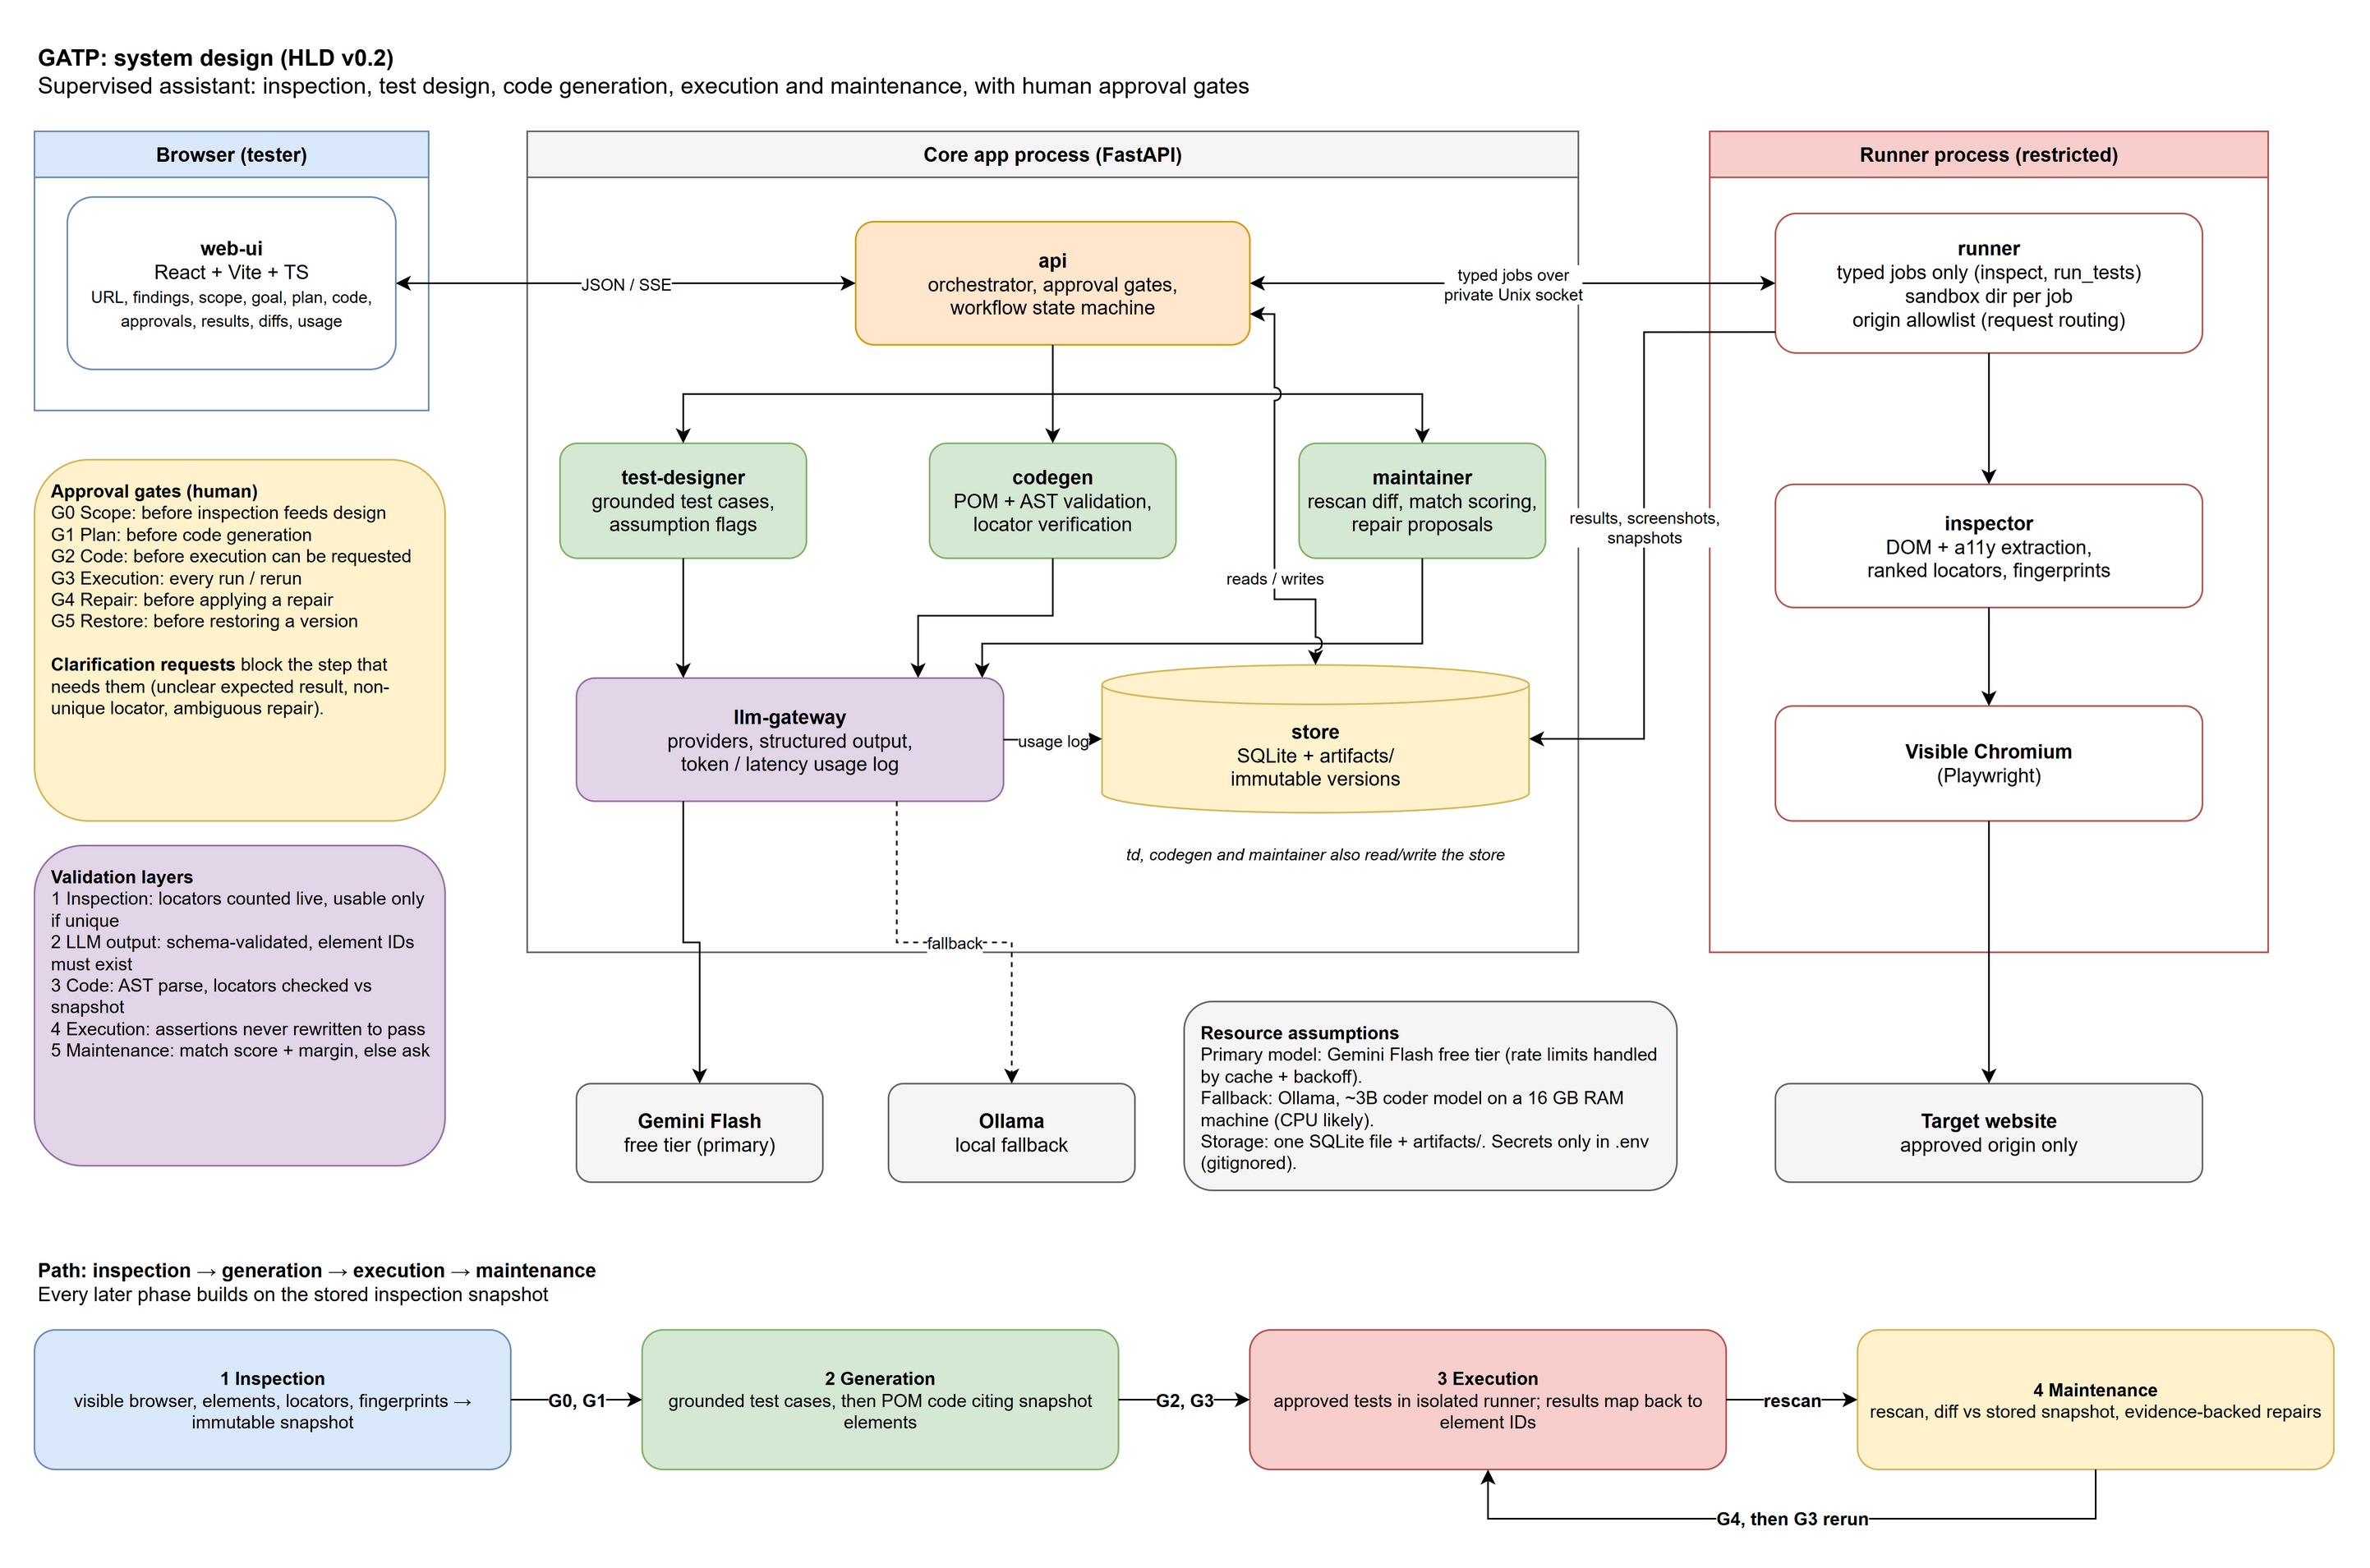
\includegraphics[width=\linewidth,height=0.9\textheight,keepaspectratio]{GATP-system-design.png}
  \caption{GATP system design: components and process boundaries, approval gates, validation layers, resource assumptions, and the path from inspection to generation, execution and maintenance.}
  \label{fig:system}
\end{figure}
\end{landscape}
\restoregeometry
\clearpage

\subsection{Components}
\begin{tabularx}{\linewidth}{@{}L{2.9cm}X@{}}
\toprule
\textbf{Module} & \textbf{Responsibility} \\
\midrule
Web interface & URL entry, findings linked to the screenshot and source line, element selection, goal and requirements, plan editor, code review, approvals, results, diffs, usage display. \\
API & HTTP and event API, workflow state machine, approval gates, clarification requests, job dispatch to the runner. \\
Inspector & Extracts interactive elements with labels, attributes, accessibility role and name; ranks candidate locators and counts each one on the live page; computes element fingerprints. \\
Store & SQLite schema, repositories, immutable versioning, artifact files. \\
LLM gateway & One entry point for model calls: provider abstraction (Gemini, Ollama), structured output, prompt templates, retries and back-off, response cache, token and latency log. \\
Test designer & Proposes grounded test cases, tags observations versus assumptions, raises clarification questions. \\
Code generation & Generates pytest-playwright Page Object code, validates it statically, checks every locator against the inspection. \\
Runner & Separate process: inspections and approved test runs in a visible browser, origin allowlist, a fresh sandbox directory per job. \\
Maintainer & Rescans, compares snapshots, scores element matches, proposes evidence-backed repairs or asks for clarification. \\
\bottomrule
\end{tabularx}

% ------------------------------------------------------------------ 3
\section{End-to-end data flow}
\label{sec:flow}
The full supervised workflow, from the first URL to a repaired and re-run test, follows one path:
\begin{enumerate}
  \item \textbf{Inspect.} The tester enters a start URL; its origin becomes the only site the browser may load. Pages that need a sign-in are reached through tester-approved setup steps (plain data such as \emph{fill}, \emph{click}), never code. The core sends an \code{inspect} job to the runner.
  \item \textbf{Findings.} The runner opens a visible browser, the inspector extracts the elements and verified locators, and the result (elements, screenshot, served HTML) is stored as an immutable inspection snapshot. The UI shows the findings linked to the screenshot and to the source line.
  \item \textbf{Scope (gate G0).} The tester sets a testing goal, includes or excludes elements, and approves the scope. Editing the scope creates a new version and reopens the gate.
  \item \textbf{Grounded model call.} Only the approved in-scope elements are sent to the model. The reply is a summary and suggested next actions, each marked as observed or assumed, plus questions for the tester. Every call is logged.
  \item \textbf{Test plan (gate G1).} The test designer proposes cases whose steps and expected results cite element ids. The tester edits, answers clarifications and approves.
  \item \textbf{Code (gate G2).} Page Object code is generated from the approved cases, validated statically and checked against the snapshot, then reviewed by the tester.
  \item \textbf{Execution (gate G3).} The tester approves running the exact tests against the approved origin. The runner executes them in a sandbox with a visible browser; results, screenshots and failure details are stored. Feedback leads to a revision and an approved rerun.
  \item \textbf{Maintenance (gate G4).} After the website changes, a rescan produces a second snapshot. The maintainer compares it with the stored one, flags changes, and proposes repairs with evidence; the tester approves a repair and the affected tests are rerun. Ambiguous cases become clarification questions instead of guesses.
\end{enumerate}

% ------------------------------------------------------------------ 4
\section{Approval gates and clarification points}
\label{sec:gates}
\begin{tabularx}{\linewidth}{@{}L{2.7cm}L{4.2cm}X@{}}
\toprule
\textbf{Gate} & \textbf{Before} & \textbf{What the tester sees} \\
\midrule
G0 Scope & the inspection is used for design & Findings list; include or exclude elements, refine the scope, set the goal. \\
G1 Plan & code generation & Test cases with actions, expected results, evidence links and assumption flags. \\
G2 Code & execution can be requested & Generated Page Objects and tests, with the validation report (syntax and locator checks). \\
G3 Execution & any run or rerun & The exact tests, the target URL, the runner limits. \\
G4 Repair & a maintenance change is applied & Old and new locator, evidence, match score, and the code diff. \\
G5 Restore & an older version is restored & The difference between the current and the target version. \\
\bottomrule
\end{tabularx}

\medskip
Each approval is stored with a timestamp, the person's name and the \emph{exact version} it applies to, so editing an item after approval invalidates the approval (an audit trail). \textbf{Clarification requests} are first-class objects: they block the step that needs them and store the question, the evidence and the tester's answer. They are raised when the expected behaviour cannot be established, when a locator is not unique, and when repair candidates are ambiguous.

% ------------------------------------------------------------------ 5
\section{Validation and grounding}
\label{sec:validation}
Five layers keep the assistant from presenting guesses as facts:
\begin{enumerate}
  \item \textbf{Inspection.} Candidate locators are ranked by Playwright's recommended priority (role and name, label, test id, placeholder or text, CSS). Each one is counted \emph{on the live page}; it is marked usable only if it matches exactly one element and that element is the target.
  \item \textbf{Model output.} Replies must be valid JSON for a schema; every element reference must resolve to an element id in the snapshot, otherwise the reply is rejected. Observations and assumptions are separate fields.
  \item \textbf{Generated code.} Python \code{ast} parsing, a static check that every locator used by a Page Object exists in the snapshot and is unique, and a pytest collection dry run in the runner.
  \item \textbf{Execution.} Assertions are never weakened or rewritten to make a test pass; failures stay visible with their evidence.
  \item \textbf{Maintenance.} A deterministic match score with a threshold and a margin; below either, the maintainer asks the tester instead of choosing.
\end{enumerate}

% ------------------------------------------------------------------ 6
\section{How later phases use inspection results}
\label{sec:later}
The inspection snapshot is the single source of truth for everything that follows.
\begin{itemize}
  \item \textbf{Test design} receives only snapshot elements and the tester's requirements; every step cites an element id.
  \item \textbf{Code generation} builds Page Objects from the snapshot's verified locators; it cannot invent selectors.
  \item \textbf{Execution} maps each failure back to the element ids involved.
  \item \textbf{Maintenance} compares the stored snapshot with a fresh one using element fingerprints rather than raw selectors.
\end{itemize}

% ------------------------------------------------------------------ 7
\section{Data model}
\label{sec:data}
State is kept in one SQLite file plus an artifacts folder. The main entities are:

\begin{tabularx}{\linewidth}{@{}L{3.6cm}X@{}}
\toprule
\textbf{Entity} & \textbf{Purpose} \\
\midrule
Project, Page & The tested site (origin = allowlist) and its pages, with their setup steps. \\
Inspection snapshot & One immutable inspection of a page: elements, screenshot, served HTML. \\
Element, Locator candidate & An observed interactive element and its ranked locators with live match counts. \\
Requirement, Clarification & Tester requirements and the questions that block a step until answered. \\
Artifact, Artifact version & Test plan, test case, Page Object, test file; every change is a new immutable version. \\
Approval & A gate decision bound to one artifact version. \\
Run, Run result & An approved execution and its per-test outcome, timings and screenshots. \\
Change set, Repair proposal & The difference between two snapshots and the evidence-backed repairs derived from it. \\
LLM call & Every model call: provider, model, version, tokens, latency, fresh or reused, and the exact request. \\
\bottomrule
\end{tabularx}

\medskip
Snapshots, locator candidates and artifact versions are immutable: the database rejects updates and deletes on them, so evidence cannot be changed after the fact.

% ------------------------------------------------------------------ 8
\section{Security and isolation}
\label{sec:security}
\begin{itemize}
  \item The runner is a separate operating-system process with its own entry point; the core application never starts a browser.
  \item It accepts only typed jobs (\code{inspect}, \code{run\_tests}) over a private Unix socket, never shell commands.
  \item Browser requests are routed through Playwright, and any request outside the approved origin is aborted.
  \item Each test run gets a fresh sandbox directory; approved test code runs inside an additional sandbox (bubblewrap) with the host's secrets hidden, and results are copied back to the artifacts folder.
  \item Page text reaches the model only inside clearly delimited data fields marked as untrusted; model output is schema-validated and never executed directly.
  \item Secrets (API keys) live only in a local \code{.env} file that is never committed; a documented \code{.env.example} lists every setting.
\end{itemize}

% ------------------------------------------------------------------ 9
\section{Model integration and resource assumptions}
\label{sec:resources}
All model calls go through the LLM gateway, which provides a common interface for the providers, schema-validated structured output, retries with back-off for rate limits, a response cache that reuses identical requests (marked \emph{reused}, with no new model call), and a log of every call.

\subsection{Configuration}
\begin{tabularx}{\linewidth}{@{}L{4.2cm}X@{}}
\toprule
\textbf{Item} & \textbf{Setting} \\
\midrule
Primary model & Google Gemini, free-tier API (default \code{gemini-3.5-flash-lite}; \code{gemini-3.5-flash} also used). \\
Fallback model & Ollama running locally (\code{qwen2.5-coder:3b}), used if the primary fails. \\
Offline mode & A deterministic \code{fake} provider for tests and offline demonstrations; the interface labels it as such. \\
Timeout and retries & 120\,s per call, with retries and back-off on rate limits. \\
Machine & Windows 11 machine running Ubuntu 24.04 under WSL2 (visible browser through WSLg); no local GPU is needed because the primary model is hosted. \\
Software & Python 3.12, FastAPI, SQLite, React/Vite/TypeScript, Playwright (Chromium), pytest. \\
Storage & One SQLite file plus an artifacts folder; deleting the data folder resets the system. \\
\bottomrule
\end{tabularx}

\subsection{Feasibility evidence: logged model calls}
Both calls summarise the approved in-scope elements of the supplied BookShelf fixture site. Tokens are those reported by the provider; model time is measured separately from browser time.

\begin{tabularx}{\linewidth}{@{}L{4.9cm}L{2.2cm}L{2.3cm}L{1.9cm}X@{}}
\toprule
\textbf{Model} & \textbf{Input tokens} & \textbf{Output tokens} & \textbf{Model time} & \textbf{Same request again} \\
\midrule
\code{gemini-3.5-flash} & 2\,433 & 1\,437 & 69.3\,s & reused, no model call \\
\code{gemini-3.5-flash-lite} & 2\,419 & 557 & 4.6\,s & reused, 0\,ms \\
\bottomrule
\end{tabularx}

\medskip
The output size and the time differ because the two runs used different models; both are real calls to the free-tier API. A tiny connectivity call (136 input and 10 output tokens) is also logged for each model. The usage log, with the exact request of every call, is delivered as a JSON file with this submission.

\subsection{Practical limits}
Free-tier latency varies from a few seconds to about 70 seconds per call, and the service can return transient errors; the gateway therefore caches identical requests, retries with back-off, and can fall back to the local model. The visible Chromium window and a local model must fit on the demonstration machine together, which is why the fallback is a small (about 3B parameter) coder model.

% ------------------------------------------------------------------ 10
\section{Implementation status and limitations}
\label{sec:status}
\begin{tabularx}{\linewidth}{@{}L{5.6cm}L{2.2cm}X@{}}
\toprule
\textbf{Area} & \textbf{Status} & \textbf{Notes} \\
\midrule
Inspection in a separate runner (visible browser, allowlist, sandbox, setup steps) & Done & Verified on the fixture site, including a page behind a sign-in. \\
Findings UI, goal and scope selection, gate G0 & Done & Findings link to the screenshot highlight and the served source line. \\
Store: immutable snapshots and versioned artifacts & Done & Diff and restore available through the API. \\
Approval gates bound to versions, clarifications & Done & Editing an approved item reopens its gate. \\
LLM gateway, validation, cache, usage log & Done & Real calls to the Gemini free tier logged. \\
Grounded model call and usage display & Done & Section~\ref{sec:resources}. \\
Test design, code generation, supervised execution, feedback, rescan and diff & Early & Implemented ahead of Phase~2; not part of the Phase~1 scope. \\
Repairs, version history view, session usage panel & Planned & Phase~2. \\
\bottomrule
\end{tabularx}

\medskip
\textbf{Quality checks.} The backend has 142 automated tests, strict type checking and lint, and the frontend passes lint and a production build. A recorded walkthrough drives the real user interface against the real runner and model.

\textbf{Known limitations.}
\begin{itemize}
  \item The platform is Linux (Windows through WSL2); the visible browser needs a display (WSLg or a virtual display).
  \item Free-tier model latency is variable and the service may fail transiently; the local fallback model is lower quality.
  \item The local fallback model has not yet been exercised in the recorded demonstration.
  \item Each page is inspected separately, and protected pages need tester-approved setup steps.
\end{itemize}

\end{document}
